%%%%%%%%%%%%%%%%%%%%%%%%%%%%%%%%%%%%%%%%%%%%%%%%%%%%%%%%%%%%%%%%%%% 
%                                                                 %
%                           CHAPTER 4                             %
%                                                                 %
%%%%%%%%%%%%%%%%%%%%%%%%%%%%%%%%%%%%%%%%%%%%%%%%%%%%%%%%%%%%%%%%%%% 
 
\chapter{The tropopause-layer static stability structure of tropical cyclones: Idealized modeling}
\resetfootnote %this command starts footnote numbering with 1 again.

%---------------------------------------------------------------------------------------%
\section{Introduction}
%---------------------------------------------------------------------------------------%

The preceding two chapters highlighted the effect of tropical cyclones on the tropopause and upper-level static stability structure in dropsonde observations.
These observations alone, however, cannot explain the mechanisms that force the observed variability.
Numerical simulations of an axisymmetric hurricane conducted in an idealized framework reproduced the observed variability.
Using these simulations, some physical insight into these mechanisms is obtained and described in the present chapter.

%---------------------------------------------------------------------------------------%
\section{Model Setup}
%---------------------------------------------------------------------------------------%

The numerical simulations were performed using version 19.4 of Cloud Model 1 (CM1) described in \cite{BryanRotunno2009}.
The equations of motion were integrated on a 3000-km-wide, 30-km-deep axisymmetric grid with 1-km horizontal and 250-m vertical grid spacing.
The computations were performed on an \textit{f}-plane at 15\textdegree{N} latitude, over a sea surface with constant temperature of 30.5\textdegree C, which matches that observed near Hurricane Patricia (2015; \citeauthor{Kimberlainetal2016} \citeyear{Kimberlainetal2016}).
Horizontal turbulence was parameterized using the Smagorinsky scheme described in \citeauthor{BryanRotunno2009} (\citeyear{BryanRotunno2009}, pg. 1773), with a prescribed mixing length that varied linearly from 100 m at a surface pressure of 1015 hPa to 1000 m at a surface pressure of 900 hPa.
Vertical turbulence was parameterized using the formulation of \citeauthor{MarkowskiBryan2016} (\citeyear{MarkowskiBryan2016}, their Eq. 6), using an asymptotic vertical mixing length of 100 m.
A Rayleigh damping layer was applied outside of the 2900-km radius and above the 25-km level to prevent spurious gravity wave reflection at the model boundaries.
Microphysical processes were parameterized using the \cite{Thompson} scheme and radiative heating tendencies were computed every two minutes using the Rapid Radiative Transfer Model for GCMs (RRTMG) longwave and shortwave schemes \citep{Iacono}.
The initial temperature and humidity field was horizontally homogeneous and determined by averaging all Climate Forecast System Reanalysis (CFSR) grid points within 100 km of Patricia's center of circulation at 18 UTC 21 October 2015.
%A horizontally-homogeneous temperature and humidity field was initialized with a mean sounding computed using all dropsondes deployed during the TCI flight conducted within and around Tropical Storm Patricia on 21 October, 2015 (see \citeauthor{DoyleTCI} \citeyear{DoyleTCI} for details.)
%Above 19 km, where few TCI observations were available, the temperature profile was taken from the Climate Forecast System Reanalysis (CFSR) grid point nearest Patricia's storm center, valid at 18 UTC 21 October, 2015.
%Since relative humidity measurements were unreliable at temperatures below -40\textdegree C \citep{BellTCI}, relative humidity was set equal to 50\% above 11.5 km (the level above which temperature dropped below -40\textdegree C).
The vortex described in \citeauthor{RotunnoEmanuel} (\citeyear{RotunnoEmanuel}, their Eq. 37) was used to initialize the wind field, setting all parameters equal to the values used therein.

Although hurricanes simulated in an axisymmetric framework tend to be more intense than those observed in nature, the intensity evolution of this simulation matches reasonably well with that observed in Hurricane Patricia.
After an initial spin-up period of about 20 hours, the modeled storm (Fig.~\ref{fig:vmax+pmin}, blue lines) began an RI period that lasted approximately 30 hours.
After this RI, the storm continued to intensify more slowly until the maximum 10-m wind speed reached 89 m s\textsuperscript{-1} and the sea-level pressure reached its minimum of 846 hPa 81 hours into the simulation.
Hurricane Patricia (red stars) exhibited a similar intensity evolution prior to its landfall, with an RI period leading to a maximum 10-m wind speed of 95 m s\textsuperscript{-1} and a minimum sea-level pressure of 872 hPa.

% 
%As in the preceding chapters, static stability is analyzed using N2, which is output directly by the model. Potential temperature tendencies 

%---------------------------------------------------------------------------------------%
\section{Results}
%---------------------------------------------------------------------------------------%

%FIGURE 1%
\begin{figure}[ht]
\centerline{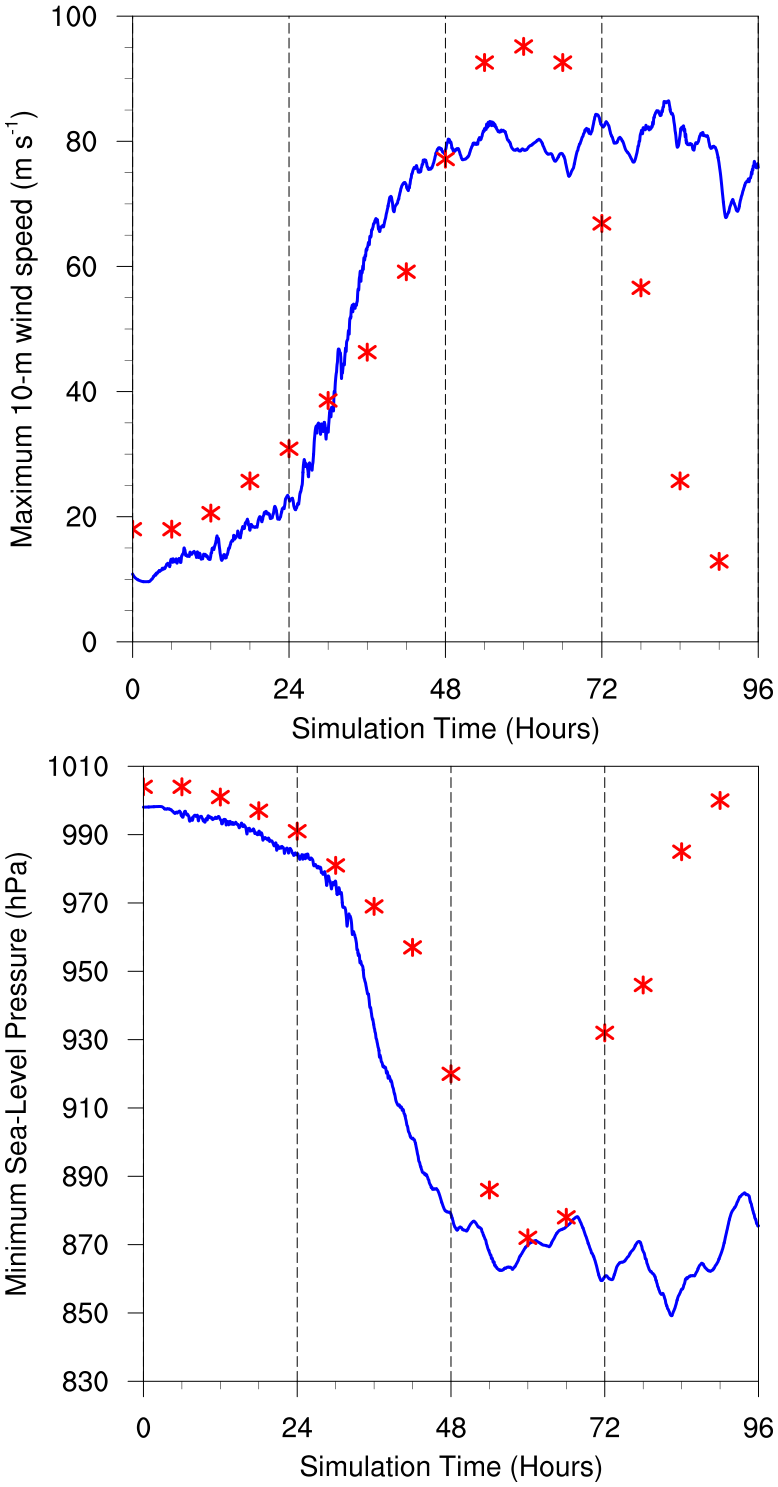
\includegraphics[width=19pc]{figures/vmax+pmin.png}}
\caption{The maximum 10-m wind speed (top panel; m s\textsuperscript{-1}) and minimum sea-level pressure (bottom panel; hPa) in the simulated storm (blue lines; plotted every minute) and from Hurricane Patricia's best track (red stars; plotted every six hours beginning at the time Patricia attained tropical storm intensity). The rapid weakening during the later stage of Patricia's lifetime was induced by landfall.}
\label{fig:vmax+pmin}
\end{figure}

